% Draft for the GSR-VLM workshop (4 pages + references).
% Generic two-column layout: swap \documentclass/preamble for the official workshop
% style file before submission. Every number here comes from results/tables.md,
% results/decomposition.json, results/elasticity.json, results/predictor.json,
% results/spatialprompt_sensitivity.json (commit 77cec95).
\documentclass[10pt,twocolumn,letterpaper]{article}
\usepackage[margin=0.75in,columnsep=0.25in]{geometry}
\usepackage{times}
\usepackage{graphicx}
\usepackage{booktabs}
\usepackage{amsmath}
\usepackage{xcolor}
\usepackage[hidelinks]{hyperref}
\usepackage[numbers,sort&compress]{natbib}
\graphicspath{{../figures/}}
\newcommand{\todo}[1]{\textcolor{red}{[TODO: #1]}}

\title{Is Scale All You're Missing?\\Metric Errors in Frozen VLMs Are Compression, Not Scale}
\author{Anonymous submission}
\date{}

\begin{document}
\maketitle

\begin{abstract}
When a frozen vision-language model (VLM) answers ``how far is the sofa from the TV?''
wrongly, is the error a misjudged scene scale, which one number could fix, or something else?
We test this on the three metric tasks of VSI-Bench with Qwen3-VL-4B. First, we split the
log-error into a part shared within a scene and a residual. The scene-shared part is small
(ICC $0.10$, 95\% CI $[0.03, 0.18]$ for absolute distance; $\approx 0$ for object size),
does not carry over across tasks, and rescaling each scene by its own mean error
\emph{lowers} accuracy. Second, the dominant error is \emph{magnitude compression}: answers grow
roughly as $\text{gt}^{0.5}$ for distances and room sizes, overestimating small quantities and
underestimating large ones. Third, we give the model metric cues in the prompt (a depth estimate from
MapAnything, a predicted scale, or the ground-truth size of another object in the scene)
and multiply each cue by $k \in [0.5, 2]$. The answers do not move: the median scale elasticity is
$0.00$ and 96--99\% of questions ignore a fourfold change of the cue. A cheap scale
predictor on the VLM's own vision tokens is accurate (median $|\log|$ error $0.08$ vs.\ $0.19$ for a
constant), so scale is available but unusable through text. Metric gains will have to come
from changing the model, not from telling it the scale.
\end{abstract}

\section{Introduction}
VLMs remain weak at metric spatial questions: on VSI-Bench~\cite{yang2025thinking},
Qwen3-VL-4B reaches 44.7 MRA on absolute distance in our setup. Recent methods
improve it with tool pipelines~\cite{seeingnotmeasuring}, fused 3D features~\cite{fan2025vlm3r},
or fine-tuned scale and depth heads~\cite{robotracer,densedepthvlm}. They change many things at once,
so it is unclear \emph{which} error they fix. Every metric answer factors as
\emph{scale $\times$ relative geometry}. If frozen VLMs mostly misjudge the scale of a scene,
a single number per scene, cheap to estimate, should recover much of the gap.

We test this hypothesis directly on a frozen model and find it false, in three ways:
\begin{enumerate}\itemsep0pt
\item \textbf{No scene-level scale error.} Only $\sim$10\% of the log-error variance in absolute distance is shared
within a scene. Scene-shared error does not correlate across tasks, and an oracle per-scene rescaling hurts.
\item \textbf{Magnitude compression.} The slope of $\log$ prediction on $\log$ ground truth is $0.54$ for
distance and $0.52$ for room size (object size: $0.87$). Most of the error is this compression.
\item \textbf{Scale cues are ignored.} We define \emph{scale elasticity}, the slope of $\log$ answer on
$\log$ hint multiplier. It is $0.00$ for every cue and task, including an oracle object size from the same scene.
\end{enumerate}

\section{Related work}
\textbf{Metric spatial reasoning.} VSI-Bench~\cite{yang2025thinking} and its cleaned rebuild ReVSI~\cite{revsi}
measure metric estimates from video. Tool-augmented agents~\cite{seeingnotmeasuring} raise absolute
distance MRA substantially and find object size limited by the 3D detector.
VLM-3R~\cite{fan2025vlm3r} fuses reconstruction tokens and notes that geometry models lack metric scale;
UniMetric~\cite{unimetric} recovers it for geometry foundation models. RoboTracer~\cite{robotracer} and
dense-depth VLMs~\cite{densedepthvlm} fine-tune scale or depth heads. All of these modify the model or its inputs.
We keep it frozen and \emph{measure} which error dominates.
\textbf{Diagnosis.} Bhat and Yamasaki~\cite{consistentyetwrong} show that spatial VLMs give view-stable but wrong answers
(``evidence insensitivity'') when the \emph{visual} evidence changes; we find the analogous insensitivity to
\emph{textual} scale evidence. SpatialPrompt~\cite{liao2024reasoning} elicits reference-object reasoning
and helps large proprietary models; we use it as a prompting baseline.

\section{Setup}
\textbf{Data.} VSI-Bench numeric tasks: absolute distance (m), object size (cm, longest dimension), room size (m$^2$);
2{,}075 questions over 288 indoor scenes. We split scenes 60/40 (seed 0, stratified by source):
173 train scenes (used only for the scale predictor) and 115 eval scenes (334/387/115 questions).
The decomposition uses all scenes.
\textbf{Model.} Qwen3-VL-4B-Instruct, frozen, greedy decoding. It receives 16 uniformly sampled frames as images
(448\,px longest side) and the official answer instruction. Unparseable answers score 0; at most 1.5\%
of answers per condition are unparseable (10\% for SpatialPrompt; see \S\ref{sec:results}).
\textbf{Metric.} Mean relative accuracy (MRA)~\cite{yang2025thinking} over thresholds $0.50{:}0.05{:}0.95$.
All CIs are 95\% scene-level bootstraps (1{,}000 resamples).

\section{Method}
\textbf{Decomposition.} For each answer, $e=\log(\hat y/y)$. We report (i) the one-way ICC of $e$ by scene,
both raw and after regressing out $\log y$, because answers that collapse to a default value make large
scenes look jointly ``scaled down'' and inflate a raw ICC; (ii) MRA after an oracle
\emph{scene} rescaling $\hat y/\exp(\bar e_{s,-i})$, using the mean error of the \emph{other} questions in the same scene;
we compare it with a \emph{global} rescaling by the mean error of all other scenes, so that a task-level bias is not
credited to scene scale; (iii) Spearman correlation of scene-mean residuals across tasks.
\textbf{Compression.} We use the slope $b$ of $\log\hat y$ on $\log y$: $b{=}1$ means proportional answers, $b{=}0$ a constant
answer. Noise in the labels biases $b$ downward. The reverse-regression value $1/\text{slope}(\log y \text{ on } \log\hat y)$
bounds it from above if all scatter were label noise.
\textbf{Scale cues.} One line is prepended to the question:
\emph{teacher}: ``the typical distance from the camera to visible surfaces is about $X$\,m'', with $X$ the
median metric depth from MapAnything~\cite{keetha2025mapanything} on the same frames (its point-cloud extent has
Spearman $0.80$ with $\sqrt{\text{room area}}$ ground truth);
\emph{teacher\_ext}: the same plus the scene extent;
\emph{learned}: $X$ from a predictor trained on the VLM's own vision tokens to regress the teacher value (train scenes only);
\emph{anchor}: the ground-truth longest dimension of a \emph{different} object in the same scene, never one named in the question;
controls are \emph{placebo} (a hint line without a number) and \emph{shuffled} (a teacher value from another scene).
\textbf{Elasticity.} We multiply the teacher and anchor values by $k\in\{0.5,0.71,1,1.41,2\}$ and fit
$\beta=\mathrm{d}\log\hat y/\mathrm{d}\log k$ per question. $\beta{=}1$ means full use of the cue and $\beta{=}0$ means it is ignored.

\section{Results}\label{sec:results}
\begin{table}[t]
\centering\small
\caption{Error decomposition of the frozen baseline (all scenes). Compression slope: $\log\hat y$ on $\log y$,
with the reverse-regression bound. MRA ($\times$100) after rescaling by the mean error of other scenes (global)
or of other questions in the same scene (scene).}
\label{tab:decomp}
\setlength{\tabcolsep}{3pt}
\begin{tabular}{lccc}
\toprule
 & Abs.\ dist. & Obj.\ size & Room size \\
\midrule
$n$ questions & 834 & 953 & 288 \\
Slope $b$ [CI] & .54 [.48,.60] & .87 [.85,.90] & .52 [.48,.56] \\
Reverse bound & 1.46 & 1.02 & 0.69 \\
ICC raw [CI] & .10 [.03,.18] & $-$.06 [$-$.11,.00] & -- \\
ICC resid.\ [CI] & .13 [.06,.21] & $-$.08 [$-$.13,$-$.03] & -- \\
MRA baseline & 44.9 & 72.9 & -- \\
\quad global rescale & 44.1 & 72.0 & -- \\
\quad scene rescale & 41.5 & 64.6 & -- \\
\bottomrule
\end{tabular}
\end{table}

\textbf{There is no scene-level scale error (Table~\ref{tab:decomp}).} For absolute distance, the scene-shared
share of error is $0.10$ ($0.13$ after removing the dependence on $\log y$), and for object size it is indistinguishable from zero.
The oracle scene rescaling, which uses ground truth, \emph{lowers} MRA (44.9$\to$41.5 for distance, 72.9$\to$64.6 for size):
the within-scene mean error is mostly noise, not a stable scene factor. Scene-mean residuals barely correlate across
tasks (distance--size $-0.07$, distance--room $0.24$, size--room $0.05$), so the scenes are not consistently
over- or under-scaled. Rooms contribute one question each, so room size is not decomposed.
The decision does not depend on hardware: an independent fp16 run on a T4 gave ICC $0.097$ against $0.104$ here (bf16).

\textbf{The error is compression.} Answers for distance and room size grow as $y^{\approx 0.5}$: short distances
and small rooms are overestimated, long ones underestimated (e.g.\ a 46.7\,m$^2$ room is answered as 20\,m$^2$).
Object size, which semantic size priors cover, is nearly proportional ($b{=}0.87$) and has the highest MRA.
For room size the compression survives the label-noise bound ($b\le0.69$). For distance the bound is
loose ($1.46$) because the model's own answers are noisy, so label noise alone cannot be excluded there.
ReVSI's relabeled distances~\cite{revsi} would settle it.

\begin{table}[t]
\centering\small
\caption{Eval scenes: MRA ($\times$100), paired change vs.\ the baseline on the same questions [95\% CI], and compression slope $b$.
Anchor covers questions with an eligible anchor object (306/369/113); the baseline slope on that subset is .55/.88/.52.
SpatialPrompt: 100 questions per task.}
\label{tab:hints}
\setlength{\tabcolsep}{2.5pt}
\begin{tabular}{lcccccc}
\toprule
 & \multicolumn{2}{c}{Abs.\ dist.} & \multicolumn{2}{c}{Obj.\ size} & \multicolumn{2}{c}{Room size} \\
 & $\Delta$MRA & $b$ & $\Delta$MRA & $b$ & $\Delta$MRA & $b$ \\
\midrule
Baseline (MRA) & 44.7 & .59 & 72.8 & .88 & 50.3 & .52 \\
Placebo & $-$0.2 & .54 & $-$0.3 & .90 & $-$0.4 & .52 \\
Shuffled & $-$0.2 & .55 & $-$0.5 & .88 & $-$0.3 & .54 \\
Teacher & $+$0.3 & .55 & $-$0.7 & .89 & $+$1.5 & .57 \\
Teacher + extent & $-$1.2 & .58 & $-$0.3 & .89 & $+$0.2 & .53 \\
Learned & $-$1.0 & .54 & $-$0.5 & .89 & $+$1.3 & .56 \\
Anchor (oracle) & $-$0.8 & .49 & $-$0.1 & .88 & $+$2.3 & .56 \\
SpatialPrompt & $-$10.4 & .38 & $-$24.6 & .50 & $-$19.8 & .68 \\
\bottomrule
\end{tabular}
\end{table}

\begin{figure}[t]
\centering
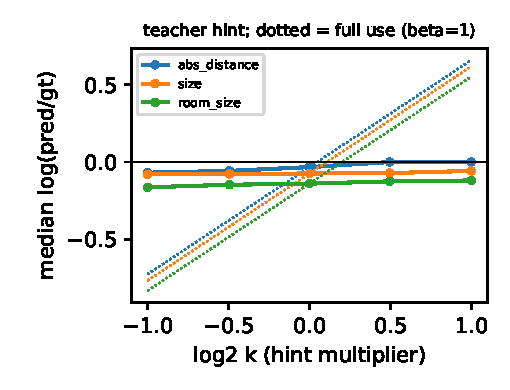
\includegraphics[width=0.49\linewidth]{elasticity_teacher.pdf}\hfill
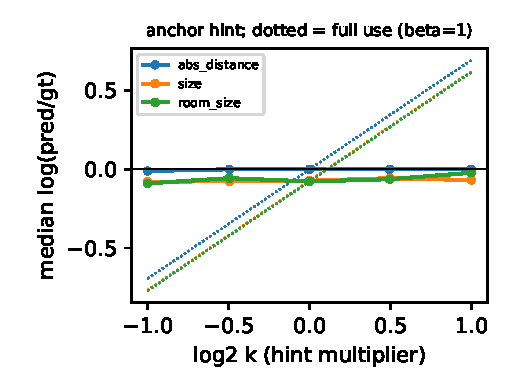
\includegraphics[width=0.49\linewidth]{elasticity_anchor.pdf}
\caption{Scale elasticity. Median $\log(\hat y/y)$ as the hint is multiplied by $k$ (left: teacher depth;
right: oracle object size). Dotted lines: full use ($\beta{=}1$). The answers are flat.}
\label{fig:elast}
\end{figure}

\textbf{Metric cues do not help (Table~\ref{tab:hints}).} Every paired change for teacher, teacher + extent,
learned and anchor is within $\pm$2.3 points, and every CI includes zero. The slope $b$ does not move toward 1 either. The oracle anchor, which tells the model the true size of
another object in the scene, is no better than the shuffled control.
SpatialPrompt hurts on every task. Part of this comes from greedy repetition loops (22/300 answers, mostly object size, still
looping at 2{,}048 tokens), but excluding them leaves $-10.4$, $-18.7$ and $-19.6$ points.

\textbf{The model ignores the cue (Fig.~\ref{fig:elast}).} The median elasticity is $0.00$ for both cues on all three tasks
(CIs within $[-0.00, 0.03]$). Between 96.1\% and 99.2\% of questions have $\beta<0.2$, and at most 0.5\% have $\beta>0.8$.
Quadrupling the cue ($k{=}0.5$ vs.\ $k{=}2$) leaves the raw answer string identical for 64\% of questions
(anchor 508/788, teacher 533/836). Copying is rare: at most 14\% of answers fall within 5\% of the hint value,
with no consistent trend across $k$.

\textbf{Scale is cheap to obtain.} A ridge probe (2.6k parameters) on the mean-pooled vision tokens of
the frozen VLM predicts the teacher scale on held-out scenes with median $|\log|$ error $0.083$, against
$0.185$ for a constant. A 1.7M-parameter frame transformer reaches $0.095$ and trains in 22\,s for three seeds.
The vision tokens carry scene scale; the text interface cannot carry it to the answer.

\section{Discussion}
For a frozen VLM, the scene-scale hypothesis fails twice: the model does not misjudge the scale of a scene,
and it does not use scale when told. What remains is a compressed mapping from perceived size to a number. This points
research toward calibrating the numeric readout, or fine-tuning scale into the model as scale-token
methods~\cite{robotracer} do, rather than toward better scale estimators feeding a prompt.
Insensitivity to text cues mirrors the evidence insensitivity reported for viewpoint changes~\cite{consistentyetwrong}.

\textbf{Limitations.} One model (Qwen3-VL-4B); cues only through text; frames given as images rather than video;
VSI-Bench labels, which are known to be noisy~\cite{revsi}, leave the distance compression estimate open to a label-noise
explanation; indoor scenes only. A null elasticity shows the model does not \emph{use} textual scale. It does not
show the model lacks internal scale, and our probe suggests it has it.

\bibliographystyle{plainnat}
\bibliography{refs}
\end{document}
